\item \textbf{{[}YIJC/PRELIM/9569/2021/P2/Q4{]} }

Lessonology is a learning management system that utilises gamification
elements to motivate students to complete their assignments. The Linked
List data structure is used to store the students\textquoteright{}
names and their total experience points. Each node contains a student\textquoteright s
name, the student\textquoteright s total experience points, and a
pointer to the next node. The nodes are linked together according
to the order provided in the \texttt{DATA.txt} file. 

A program is to be written to implement nodes as an instance of the
class \texttt{Node}. The class \texttt{Node} has the following properties
and method: 
\begin{center}
\begin{tabular}{|l|l|}
\hline 
\multicolumn{2}{|c|}{\texttt{Class: Node}}\tabularnewline
\hline 
\multicolumn{2}{|c|}{Properties}\tabularnewline
\hline 
\texttt{\hspace{0.01\columnwidth}}Identifier & \texttt{\hspace{0.05\columnwidth}}Description\tabularnewline
\hline 
\texttt{Name} & The node\textquoteright s value for a student\textquoteright s name.\tabularnewline
\hline 
\texttt{Exp} & The node\textquoteright s value for the student\textquoteright s total
experience points.\tabularnewline
\hline 
\texttt{Pointer} & The pointer to the next node.\tabularnewline
\hline 
\multicolumn{2}{|c|}{Method}\tabularnewline
\hline 
\texttt{\hspace{0.01\columnwidth}}Identifier & \texttt{\hspace{0.05\columnwidth}}Description\tabularnewline
\hline 
\texttt{SetPointer()} & Set the pointer to point at the next node or point to \texttt{None}
when it is the last node.\tabularnewline
\hline 
\end{tabular}
\par\end{center}

A linked list is implemented as an instance of the class \texttt{StudentList}.
The class \texttt{StudentList} has the following property and methods: 
\noindent \begin{center}
\begin{tabular}{|l|l|}
\hline 
\multicolumn{2}{|c|}{\texttt{Class: StudentList}}\tabularnewline
\hline 
\multicolumn{2}{|c|}{Properties}\tabularnewline
\hline 
\texttt{\hspace{0.01\columnwidth}}Identifier & \texttt{\hspace{0.05\columnwidth}}Description\tabularnewline
\hline 
\texttt{Start} & The pointer at the start of the linked list.\tabularnewline
\hline 
\multicolumn{2}{|c|}{Methods}\tabularnewline
\hline 
\texttt{\hspace{0.01\columnwidth}}Identifier & \texttt{\hspace{0.05\columnwidth}}Description\tabularnewline
\hline 
\texttt{Constructor} & Initialise the linked list with the pointer \texttt{Start} assigned
to \texttt{None}.\tabularnewline
\hline 
\texttt{Add()} & Add a new node into the linked list.\tabularnewline
\hline 
\texttt{Update()} & Update the value for the total experience points of a student\textquoteright s
node in the linked list.\tabularnewline
\hline 
\texttt{Delete()} & Delete a node in the linked list.\tabularnewline
\hline 
\texttt{Display()} & Display the current content of the linked list in table form.\tabularnewline
\hline 
\end{tabular}
\par\end{center}

\subsubsection*{Task 4.1 }

Write program code for the classes \texttt{Node} and \texttt{StudentList},
including the \texttt{Constructor},\texttt{ Add() }and \texttt{Display()}
methods. The code should follow the specification given. Do not write
the \texttt{Update()} and \texttt{Delete()} methods yet. 

The \texttt{Add(node)} method for the \texttt{StudentList} class should
add the \texttt{node} containing a student\textquoteright s name and
the student\textquoteright s total experience points to the linked
list, according to the order given in the \texttt{DATA.txt} file. 

Test your code by reading the data from the file \texttt{DATA.txt}
and adding them as nodes into the linked list. The diagram below shows
a portion of the expected output when using the \texttt{Display()}
method on the populated linked list: 
\noindent \begin{center}
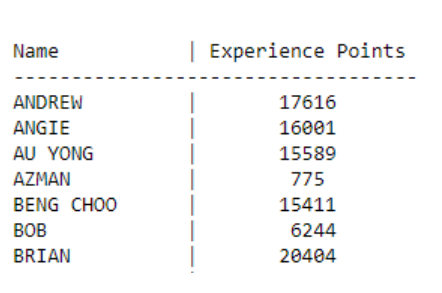
\includegraphics[scale=0.5]{C:/Users/Admin/Desktop/Github/question_bank/LyX/static/img/9569-YIJC-2021-P2-Q4-1}
\par\end{center}

\hfill{}{[}9{]}

\subsubsection*{Task 4.2 }

Each time a student completes an assignment, points will be awarded
and the student\textquoteright s total experience points will be updated. 

Write program code for the \texttt{Update(name,points)} method for
the \texttt{StudentList} class that takes a student\textquoteright s
\texttt{name} and the awarded \texttt{points} as inputs to update
the student\textquoteright s total experience points in the node.
(You may assume that the node containing the student exists in the
linked list.) 

For example, \texttt{Update('BRIAN',100)} will update the total experience
points of a student whose name is \texttt{'BRIAN'} from \texttt{20404}
to \texttt{20504}. \hfill{}{[}3{]}

\subsubsection*{Task 4.3 }

Write program code to implement the \texttt{Delete(name)} method for
the \texttt{StudentList} class to search and remove a node, containing
a particular student\textquoteright s \texttt{name}, in the linked
list. Return \texttt{True} if the node is found and removed; otherwise
return \texttt{False}. (You may assume that the students\textquoteright{}
names are unique in the linked list.) \hfill{}{[}4{]}

\subsubsection*{Task 4.4 }

Another linked list which has pointers linking the nodes in decreasing
order of the experience points is implemented as an instance of the
class \texttt{Leaderboard}. 

The class \texttt{Leaderboard} has the following properties and methods: 
\noindent \begin{center}
\begin{tabular}{|l|l|}
\hline 
\multicolumn{2}{|c|}{\texttt{Class: Leaderboard}}\tabularnewline
\hline 
\multicolumn{2}{|c|}{Properties}\tabularnewline
\hline 
\texttt{\hspace{0.01\columnwidth}}Identifier & \texttt{\hspace{0.05\columnwidth}}Description\tabularnewline
\hline 
\texttt{Start} & The pointer at the start of the linked list.\tabularnewline
\hline 
\multicolumn{2}{|c|}{Methods}\tabularnewline
\hline 
\texttt{\hspace{0.01\columnwidth}}Identifier & \texttt{\hspace{0.05\columnwidth}}Description\tabularnewline
\hline 
\texttt{Constructor} & Inherit the property and all the methods from the class \texttt{StudentList}.
Initialise the linked list with the pointer \texttt{Start} assigned
to \texttt{None}.\tabularnewline
\hline 
\texttt{Add()} & Modify the \texttt{Add()} method in the parent class to add a new
node in decreasing order of total experience points.\tabularnewline
\hline 
\texttt{Update()} & Modify the \texttt{Update()} method in the parent class such that
the linked list is still in decreasing order of experience points
after updating a student\textquoteright s total experience points.\tabularnewline
\hline 
\texttt{DisplayTop()} & Display the content of the nodes in the linked list for the top students
based on their total experience points.\tabularnewline
\hline 
\end{tabular}
\par\end{center}

Write program code for the class \texttt{Leaderboard} to inherit the
properties and methods from the class \texttt{StudentList} with the
modified \texttt{Add()} and \texttt{Update()} methods. The additional
\texttt{DisplayTop(n)} method should display the top \texttt{n} number
of students in the linked list, based on their total experience points.
(You may assume that no two students have the same total experience
points.) 

Test your code by reading the data from the file \texttt{DATA.txt}
and adding them as nodes into this linked list. The diagram below
shows the expected output when using the \texttt{DisplayTop(5)} method
on the linked list: 
\noindent \begin{center}
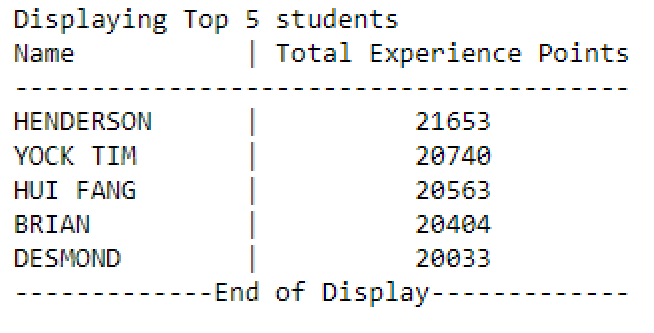
\includegraphics[scale=0.5]{C:/Users/Admin/Desktop/Github/question_bank/LyX/static/img/9569-YIJC-2021-P2-Q4-2}
\par\end{center}

\hfill{}{[}13{]}